\chapter{Lagrangian Examples and Hamilton's Equations}

The point of this lecture is practical before it is grand. Leonard Susskind wants to show, by example, that the Lagrangian formalism turns awkward constrained systems into a largely mechanical exercise: choose coordinates, write down \(L=T-V\), and let the equations organize themselves. These companion notes follow that progression closely, from two worked systems to the Hamiltonian formulation and finally to the harmonic oscillator in phase space. The supporting board captures used here were curated for this edition by LazyingArt LLC and Video2Book.

\section{Why Lagrangians Are Powerful}

The opening move is an important one. We are not promised a closed-form solution of every trajectory. Instead, we are told what it means, for present purposes, to solve a mechanics problem: write down the equations of motion. Once that is done, one may always hand the resulting differential equations to a computer. The hard part, in many nontrivial systems, is not the final integration but the correct setup.

This is exactly the sort of thing for which the Lagrangian is good. One does not chase every contact force and constraint force separately. One chooses coordinates that describe the instantaneous configuration, writes \(T\) and \(V\), and then the Euler--Lagrange equations follow.

\subsection{Question \& Answer}

\paragraph{Question.} What does it mean to solve a mechanics problem here?

\paragraph{Answer.} In this lecture, it means finding the equations of motion. If one can write those equations down cleanly, the mechanical problem is already under control, even if the explicit trajectories are later obtained numerically rather than in closed form.

\section{Sliding Wedge: Coordinates, \texorpdfstring{$T-V$}{T-V}, and Canonical Momentum}

The first example is a wedge of mass \(M\) constrained to slide horizontally without friction, together with a point particle of mass \(m\) constrained to move along the hypotenuse. Susskind first emphasizes the general rule: the coordinates are not unique, but they must be sufficient and nonredundant.

For the lecture he chooses two horizontal coordinates:
\[
X=\text{horizontal position of the wedge corner},\qquad
x=\text{horizontal position of the particle relative to that corner}.
\]
To keep the algebra clean he then specializes to a \(45^\circ\) wedge, so that
\[
y=x,\qquad \dot y=\dot x.
\]
The kinetic energy of the wedge is immediate:
\begin{equation}
T_{\text{wedge}}=\frac12 M\dot X^2.
\end{equation}
For the particle, the horizontal component of velocity is \(\dot X+\dot x\), while the vertical component is \(\dot x\) in the \(45^\circ\) case. Thus
\begin{equation}
T_{\text{particle}}=\frac m2\Big[(\dot X+\dot x)^2+\dot x^2\Big].
\end{equation}
The potential energy is equally simple in this special geometry:
\begin{equation}
V=mgx.
\end{equation}
Therefore the Lagrangian is
\begin{equation}
L=\frac12 M\dot X^2+\frac m2\Big[(\dot X+\dot x)^2+\dot x^2\Big]-mgx.
\end{equation}

Now the lecture turns away from solving both Euler--Lagrange equations in detail. The interesting point is instead the meaning of canonical momentum. By definition,
\begin{align}
p_X&=\frac{\partial L}{\partial \dot X}
   =M\dot X+m(\dot X+\dot x),\\
p_x&=\frac{\partial L}{\partial \dot x}
   =m(\dot X+\dot x)+m\dot x.
\end{align}
This is where Susskind pauses. Canonical momentum is not simply the naive \(mv\) attached to whichever piece of matter one happens to be staring at. It is defined by differentiation of the Lagrangian. In constrained systems that distinction matters.

The symmetry is horizontal translation of the whole arrangement:
\begin{equation}
\delta X=\epsilon,\qquad \delta x=0.
\end{equation}
Equivalently, \(X\) is a cyclic coordinate. Hence
\begin{equation}
\dot p_X=\frac{\partial L}{\partial X}=0.
\end{equation}
This is the conservation law the lecture wants us to see. The Lagrangian formalism finds it without ever forcing us to solve explicitly for the reaction forces between wedge and particle.

For completeness, the second Euler--Lagrange equation in this \(45^\circ\) example reads
\begin{equation}
\dot p_x=\frac{\partial L}{\partial x}=-mg.
\end{equation}
Even here Susskind briefly trips over the sign and then corrects it. The safe statement is the canonical one: since \(L=T-V\), the derivative with respect to \(x\) comes entirely from \(-V\).

\section{Double Pendulum: Choosing the Right Angle Variables}

The second example is the double pendulum with unit lengths and, for simplicity, unit masses. Here the crucial point is not brute algebra; it is the choice of coordinates.

The first angle is naturally called \(\theta\). For the second rod there are two tempting conventions. One may measure it relative to the vertical, or one may measure it relative to the first rod and call the relative angle \(\alpha\). Susskind chooses the second convention, not because the other one is wrong, but because this one makes the symmetry easier to see.

If gravity is temporarily turned off, the entire system has rotational symmetry. With the relative-angle choice, that symmetry acts by
\begin{equation}
\theta\to \theta+\epsilon,\qquad \alpha\to \alpha.
\end{equation}
That is exactly the sort of action one wants. The symmetry shifts one coordinate and leaves the other fixed.

\subsection{Question \& Answer}

\paragraph{Question.} Why is \(\alpha\) measured relative to the first rod rather than relative to the vertical?

\paragraph{Answer.} Because in the no-gravity problem the global rotation symmetry then acts only on \(\theta\). That makes \(\theta\) the cyclic coordinate. Had we measured the second angle from the vertical, both angles would transform under a rotation, and the symmetry would be less transparent even though the physics would be the same.

The lecture makes a larger methodological point here. The equations of motion can be written in many coordinate systems, but not every coordinate system is equally revealing. The art lies in choosing coordinates that let symmetry act simply.

\section{Double Pendulum: Kinematics, Symmetry, and Gravity}

To compute the kinetic energy, Susskind introduces temporary Cartesian coordinates for the two bobs. For the first bob,
\begin{equation}
x=\sin\theta,\qquad y=\cos\theta,
\end{equation}
with \(y\) taken downward for convenience. Differentiating,
\begin{equation}
\dot x=\dot\theta\cos\theta,\qquad \dot y=-\dot\theta\sin\theta.
\end{equation}
Hence
\begin{equation}
\dot x^{\,2}+\dot y^{\,2}=\dot\theta^{\,2}.
\end{equation}

For the second bob one writes
\begin{equation}
x'=\sin\theta+\sin(\theta+\alpha),\qquad
y'=\cos\theta+\cos(\theta+\alpha).
\end{equation}
The resulting velocity formulas are straightforward but already a little messy; that is precisely why the Cartesian detour is helpful.

A representative step is
\begin{equation}
\dot x'=\dot\theta\cos\theta+(\dot\theta+\dot\alpha)\cos(\theta+\alpha),
\end{equation}
and a similar expression holds for \(\dot y'\). At that stage one adds the two \(v^2\) terms and rewrites everything in angular variables.

The lecture itself does not insist on a perfectly normalized final expression, and in fact the sign convention in the mixed \(\dot\theta\)--\(\dot\alpha\) terms is openly challenged from the audience. A board form visible later in the lecture is
\begin{equation}
T-V=\dot\theta^{\,2}+\frac{(\dot\theta-\dot\alpha)^2}{2}
+\dot\theta(\dot\theta-\dot\alpha)\cos\alpha,
\end{equation}
but this should be read with caution: the lecture itself treats the sign of the \(\dot\alpha\) terms as dependent on convention.

\begin{figure}[htbp]
\centering

\includegraphics[width=0.82\textwidth]{lecture_06_figure_02.png}
\caption{Double-pendulum board state. The upper line shows one lecture-local form of the kinetic terms; the lower line isolates the \(\theta\)-equation. The board writes \(P_\theta\), though we keep the notes in the standard lowercase notation \(p_\theta\).}
\end{figure}

The secure point is the symmetry statement. In the absence of gravity, \(\theta\) does not appear explicitly in the Lagrangian, so
\begin{equation}
\dot p_\theta=\frac{\partial L}{\partial \theta}=0.
\end{equation}
That conserved quantity is the total angular momentum of the two-bob system.

This is an important place where the lecture answers a natural misconception. Conservation of angular momentum does \emph{not} mean that the angular velocity of each bob is constant. The two parts of the system exchange angular momentum through the rod forces; what is conserved is the total quantity, not the individual rates \(\dot\theta\) and \(\dot\alpha\).

Once gravity is restored, the rotational symmetry is broken. The potential energy is then built from the heights of the two bobs and therefore contains a sum of cosine terms,
\begin{equation}
V_{\text{grav}}\propto \cos\theta+\cos(\theta+\alpha),
\end{equation}
up to overall sign and normalization conventions depending on how the vertical coordinate is chosen. The exact coefficients are not the main point of the lecture. The point is that gravity spoils the cyclic-coordinate argument, so the conservation law tied to free rotation disappears.

\section{Hamiltonian Mechanics as a New Formulation}

Only after those two examples does the lecture pivot to the Hamiltonian. This is not introduced as a minor reformulation. It is the third major formulation of mechanics encountered so far:
\begin{itemize}
\item Newton's equations,
\item the Lagrangian or least-action formulation,
\item the Hamiltonian formulation.
\end{itemize}

The Hamiltonian is first identified as energy. But Susskind immediately widens the scope: it is also the basis of a new way of writing the laws of motion. The new variables are not \(q_i\) and \(\dot q_i\), but \(q_i\) and \(p_i\). For a good mechanical system one should be able to solve the velocity-momentum relations and express the \(\dot q_i\) in terms of \(q_i\) and \(p_i\). Then the Hamiltonian may truly be regarded as a function \(H(q,p)\).

At this point the lecture briefly reaches back to the first day of the course. A reversible law of motion should not squeeze many states into one future state, and it should not explode one state into several futures. In the language Susskind is building toward, the flow in phase space must have neither convergence into sinks nor divergence out of sources. Hamiltonian mechanics is where that geometric statement becomes precise.

\section{Deriving Hamilton's Equations}

The defining formula is
\begin{equation}
H=\sum_i \dot q_i p_i-L.
\end{equation}
To derive the equations of motion we apply the standard multivariable variation identity,
\begin{equation}
\delta F=\sum_i\left(\frac{\partial F}{\partial q_i}\delta q_i+\frac{\partial F}{\partial p_i}\delta p_i\right).
\end{equation}
Now vary \(H\) directly, not yet assuming any explicit final formula for \(H(q,p)\):
\begin{align}
\delta H
&=\sum_i\big(\dot q_i\,\delta p_i+p_i\,\delta \dot q_i\big)
-\sum_i\left(\frac{\partial L}{\partial \dot q_i}\delta \dot q_i+\frac{\partial L}{\partial q_i}\delta q_i\right).
\end{align}
Because
\[
\frac{\partial L}{\partial \dot q_i}=p_i,
\]
the \(p_i\,\delta\dot q_i\) terms cancel. Then Euler--Lagrange gives
\[
\frac{\partial L}{\partial q_i}=\dot p_i.
\]
Thus
\begin{equation}
\delta H=\sum_i \dot q_i\,\delta p_i-\dot p_i\,\delta q_i.
\end{equation}
Comparing coefficients with the general variation formula, we read off Hamilton's equations:
\begin{equation}
\frac{\partial H}{\partial p_i}=\dot q_i,\qquad
\frac{\partial H}{\partial q_i}=-\dot p_i.
\end{equation}
This is the formal center of the lecture. The \(q\)'s and \(p\)'s now stand on almost the same footing, apart from the single minus sign.

\begin{figure}[htbp]
\centering

\includegraphics[width=0.72\textwidth]{lecture_06_figure_03.png}
\caption{Hamiltonian definition and the boxed Hamilton equations on the board. The visual hierarchy matters: derivation above, final canonical form below.}
\end{figure}

The lecture then makes a structural observation that becomes important immediately afterward. For \(n\) coordinates, the Lagrangian description gives \(n\) second-order equations. The Hamiltonian description gives \(2n\) first-order equations. The information is the same; the bookkeeping is different.

\section{The Harmonic Oscillator in Phase Space}

The harmonic oscillator is the clean example on which the new formalism is displayed. Susskind deliberately chooses a rescaled Lagrangian,
\begin{equation}
L=\frac{1}{2\omega}\dot q^{\,2}-\frac{\omega}{2}q^2,
\end{equation}
with \(\omega\) the oscillator frequency.

This form is not magic. One starts from the familiar oscillator,
\begin{equation}
L=\frac12 m\dot x^2-\frac12 kx^2,\qquad \omega=\sqrt{\frac{k}{m}},
\end{equation}
and then chooses a new coordinate \(q\) so that
\begin{equation}
\frac{\omega}{2}q^2=\frac{k}{2}x^2.
\end{equation}
Equivalently,
\begin{equation}
q^2=\sqrt{km}\,x^2,
\end{equation}
so \(q\) is no longer a physical length. That is the price of the rescaling, and the lecture spends time acknowledging it. The reward is symmetry between the \(q\) and \(p\) terms in the Hamiltonian.

The conjugate momentum is
\begin{equation}
p=\frac{\partial L}{\partial \dot q}=\frac{\dot q}{\omega},
\end{equation}
so
\begin{equation}
\dot q=\omega p.
\end{equation}
Then
\begin{equation}
H=\dot q\,p-L=\frac{\omega}{2}(p^2+q^2).
\end{equation}
This is the payoff. Constant energy means
\begin{equation}
p^2+q^2=\frac{2H}{\omega}=\text{constant},
\end{equation}
so the motion in phase space lies on circles.

\begin{figure}[htbp]
\centering

\includegraphics[width=0.74\textwidth]{lecture_06_figure_04.png}
\caption{The hand-drawn phase portrait on the board: nested closed trajectories, a marked orbit, and a cloud of starting points.}
\end{figure}

\begin{figure}[htbp]
\centering
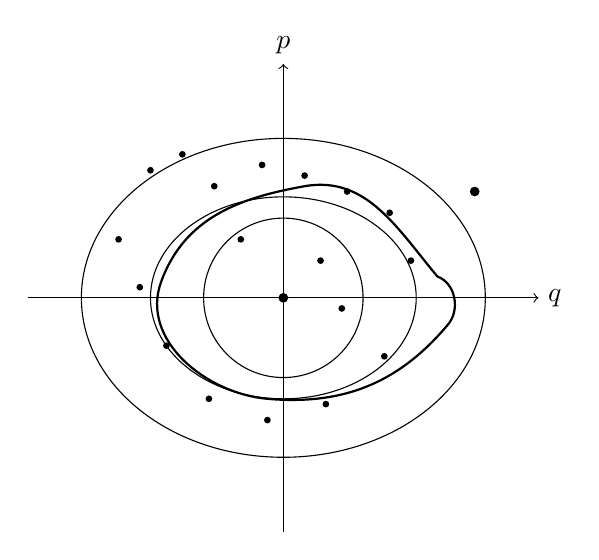
\begin{tikzpicture}[scale=1.35]
\draw[->] (-2.4,0) -- (2.4,0) node[right] {$q$};
\draw[->] (0,-2.2) -- (0,2.2) node[above] {$p$};
\draw (0,0) circle (0.75);
\draw (0,0) ellipse (1.25 and 0.95);
\draw (0,0) ellipse (1.9 and 1.5);
\draw[thick] (1.45,0.2)
  to[out=130,in=10] (0.2,1.05)
  to[out=190,in=70] (-1.15,0.15)
  to[out=-110,in=175] (-0.15,-0.95)
  to[out=-5,in=-130] (1.55,-0.25)
  to[out=50,in=-20] (1.45,0.2);
\fill (0.00,0.00) circle (1.3pt);
\fill (1.80,1.00) circle (1.3pt);
\fill (-1.25,1.20) circle (0.9pt);
\fill (-1.55,0.55) circle (0.9pt);
\fill (-0.95,1.35) circle (0.9pt);
\fill (-0.65,1.05) circle (0.9pt);
\fill (-0.20,1.25) circle (0.9pt);
\fill (0.20,1.15) circle (0.9pt);
\fill (0.60,1.00) circle (0.9pt);
\fill (1.00,0.80) circle (0.9pt);
\fill (1.20,0.35) circle (0.9pt);
\fill (0.95,-0.55) circle (0.9pt);
\fill (0.40,-1.00) circle (0.9pt);
\fill (-0.15,-1.15) circle (0.9pt);
\fill (-0.70,-0.95) circle (0.9pt);
\fill (-1.10,-0.45) circle (0.9pt);
\fill (-1.35,0.10) circle (0.9pt);
\fill (-0.40,0.55) circle (0.9pt);
\fill (0.35,0.35) circle (0.9pt);
\fill (0.55,-0.10) circle (0.9pt);
\end{tikzpicture}
\caption{A cleaned redraw of the phase-space portrait suggested on the board. The lecture's picture is not about literal geometry but about closed orbits and a fluid of starting points carried along by the Hamiltonian flow.}
\end{figure}

The lecture makes the geometric point in two complementary ways. One may think of a single initial condition moving on its circle forever. Or one may imagine many initial points, as though phase space were filled with a fictitious fluid. Then the whole cloud rotates rigidly. That is the beginning of the phase-space picture to which the next lecture will return.

\subsection{Question \& Answer}

\paragraph{Question.} If Hamilton's equations are first order and Euler--Lagrange equations are second order, how can they describe the same mechanics?

\paragraph{Answer.} For one degree of freedom, Hamilton's equations are the pair
\begin{equation}
\dot q=\omega p,\qquad \dot p=-\omega q.
\end{equation}
Differentiate the first with respect to time:
\[
\ddot q=\omega \dot p.
\]
Now substitute the second:
\begin{equation}
\ddot q=-\omega^2 q.
\end{equation}
That is exactly the usual second-order oscillator equation. The Hamiltonian formulation splits one second-order law into two coupled first-order laws.

The board later juxtaposes precisely these two ways of writing the same dynamics.

\begin{figure}[htbp]
\centering

\includegraphics[width=0.92\textwidth]{lecture_06_figure_05.png}
\caption{The oscillator written both ways on the board: phase-space motion on the left, first- and second-order equations on the right.}
\end{figure}

For comparison, the Euler--Lagrange form is
\begin{equation}
\frac{d}{dt}\!\left(\frac{\dot q}{\omega}\right)=-\omega q,
\end{equation}
or equivalently
\begin{equation}
\frac{\ddot q}{\omega}=-\omega q.
\end{equation}
Multiplying by \(\omega\) gives back the same second-order oscillator equation.

It is also worth noticing why the rescaling was introduced at all. In the original variables \((x,p_x)\), the Hamiltonian would be
\begin{equation}
H=\frac{p_x^2}{2m}+\frac{k}{2}x^2,
\end{equation}
so the energy contours would be ellipses. By passing to the adapted coordinate \(q\), Susskind makes the symmetry of the oscillator visible: the level sets are circles, and the phase-space flow is rigid rotation with angular speed \(\omega\).

\begin{figure}[htbp]
\centering
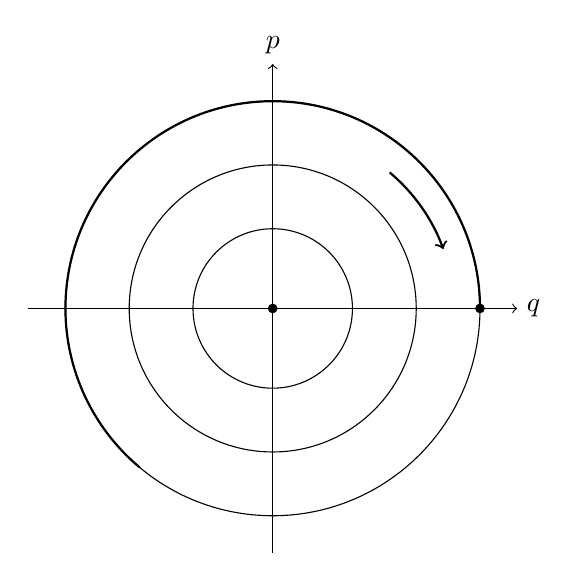
\begin{tikzpicture}[scale=1.35]
\draw[->] (-2.3,0) -- (2.3,0) node[right] {$q$};
\draw[->] (0,-2.3) -- (0,2.3) node[above] {$p$};
\draw (0,0) circle (0.75);
\draw (0,0) circle (1.35);
\draw (0,0) circle (1.95);
\draw[thick] (1.95,0) arc[start angle=0,end angle=230,radius=1.95];
\draw[->,thick] (1.10,1.28) arc[start angle=50,end angle=20,radius=1.7];
\fill (0,0) circle (1.3pt);
\fill (1.95,0) circle (1.3pt);
\end{tikzpicture}
\caption{A cleaned oscillator phase portrait. The essential content is constant-energy circles and uniform rotation, not the exact drawing style of the board sketch.}
\end{figure}

There is one further lesson in the oscillator example. To formulate the Hamiltonian theory we must be able to eliminate \(\dot q\) in favor of \(p\). The lecture makes this into a real criterion: if the velocity-momentum relation cannot be solved, then one does not have the kind of mechanical system the Hamiltonian formalism wants, and quantum mechanics will be unhappy with it as well.

\section{Summary and Outlook}

The lecture begins with the deliberately modest claim that Lagrangians make complicated constrained systems manageable, and it delivers exactly that. The wedge problem shows the method at work in its simplest form: choose coordinates, write \(T-V\), compute canonical momenta, and read off a conservation law from symmetry. The double pendulum then shows that the real intelligence often lies in the choice of coordinates, because the right coordinates make cyclic variables and conservation laws visible.

From there the Hamiltonian enters first as conserved energy and then as a new formulation of mechanics. Its equations are first order, but they encode the same dynamics as the second-order Euler--Lagrange equations. For the harmonic oscillator they reveal something the older form hides: in the right variables the motion is a rigid rotation in phase space.

The lecture closes by widening the perspective. Phase space is not simply better than configuration space; it is useful for different reasons. In particular it makes the geometry of the flow visible. One sees cycles, conserved quantities, and the absence of convergence or divergence in the fictitious phase-space fluid. That geometric clarity is one reason the Hamiltonian is beautiful. The deeper reason, Susskind insists, is that the Hamiltonian sits at the center of quantum mechanics.

Finally, the lecture returns to a foundational point about conservative mechanics. It is better to think of potential energy as primary and force as derived:
\[
F_i=-\frac{\partial V}{\partial q_i},
\]
when such a potential exists. In that form the hierarchy is clear. The Lagrangian organizes the mechanics, the Hamiltonian reorganizes it geometrically, and both are already pointing beyond classical mechanics toward the modern subjects for which this course is meant to prepare us.